\begin{frame}{Feature Engineering}

\begin{itemize}
    \item Create new features based on existing ones
    \begin{itemize}
        \item Polynomial features
        \item Interaction features
        \item Binning
    \end{itemize}

    \item Mainly useful for simple models (e.g. linear models)
    \begin{itemize}
        \item Other models can learn interactions themselves
        \item But may be slower, less robust than linear models
    \end{itemize}
\end{itemize}

\end{frame}

\begin{frame}{Polynomials}

\begin{itemize}
    \item Add all polynomials up to degree $d$ and all products
    \begin{itemize}
        \item Equivalent to polynomial basis expansions
    \end{itemize}
\end{itemize}

\[
[1, x_1, \ldots, x_p] \rightarrow [1, x_1, \ldots, x_p, x_1^2, \ldots, x_p^2, \ldots, x_p^d, x_1 x_2, \ldots, x_{p-1} x_p]
\]

\begin{center}
    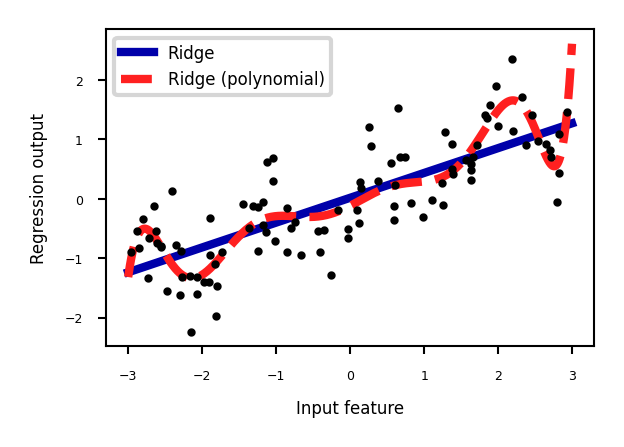
\includegraphics[width=0.75\textwidth]{images/pre-processing/polynomial.png}
\end{center}

\end{frame}



\begin{frame}[allowframebreaks]{Binning}

\begin{itemize}
    \item Partition numeric feature values into $n$ intervals (bins)
    \item Create $n$ new one-hot features, 1 if original value falls in corresponding bin
    \item Models different intervals differently (e.g. different age groups)
\end{itemize}

\begin{center}
\begin{tabular}{rcccc}
\textbf{orig} & \textbf{[-3.0,-1.5]} & \textbf{[-1.5,0.0]} & \textbf{[0.0,1.5]} & \textbf{[1.5,3.0]} \\
\hline
-0.752759 & 0.000000 & 1.000000 & 0.000000 & 0.000000 \\
 2.704286 & 0.000000 & 0.000000 & 0.000000 & 1.000000 \\
 1.391964 & 0.000000 & 0.000000 & 1.000000 & 0.000000 \\
\end{tabular}
\end{center}

\vspace{1em}

\begin{center}
    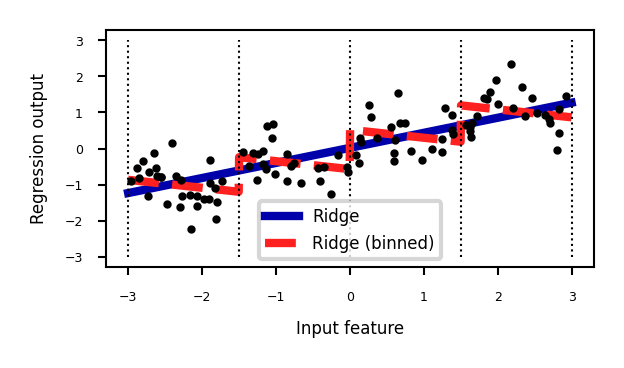
\includegraphics[width=0.75\textwidth]{images/pre-processing/binning.png}
\end{center}

\end{frame}


\begin{frame}{Binning + interaction features}

\begin{itemize}
    \item Add \textit{interaction features} (or \textit{product features})
    \begin{itemize}
        \item Product of the bin encoding and the original feature value
        \item Learn different weights per bin
    \end{itemize}
\end{itemize}

\vspace{0.5em}

\begin{center}
\resizebox{\textwidth}{!}{
\begin{tabular}{rcccccccc}
\textbf{orig} & \textbf{b0} & \textbf{b1} & \textbf{b2} & \textbf{b3} & \textbf{X*b0} & \textbf{X*b1} & \textbf{X*b2} & \textbf{X*b3} \\
\hline
-0.752759 & 0.000000 & 1.000000 & 0.000000 & 0.000000 & -0.752759 & -0.000000 & -0.000000 & -0.000000 \\
 2.704286 & 0.000000 & 0.000000 & 0.000000 & 1.000000 &  0.000000 &  0.000000 &  0.000000 &  2.704286 \\
 1.391964 & 0.000000 & 0.000000 & 1.000000 & 0.000000 &  0.000000 &  0.000000 &  1.391964 &  0.000000 \\
\end{tabular}
}
\end{center}

\vspace{1em}

\begin{center}
    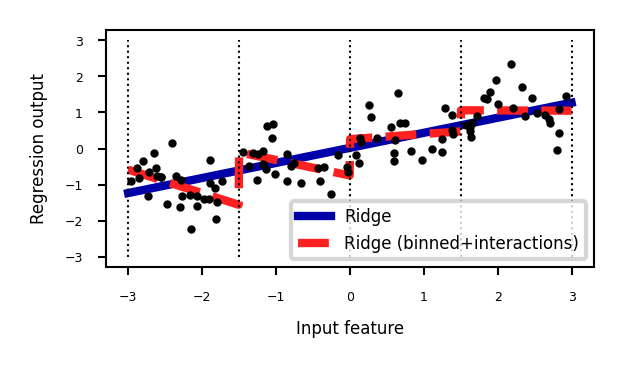
\includegraphics[width=0.75\textwidth]{images/pre-processing/binning-interactions.png}
\end{center}

\end{frame}


\begin{frame}{Categorical feature interactions}

\begin{itemize}
    \item One-hot-encode categorical feature
    \item Multiply every one-hot-encoded column with every numeric feature
    \item Allows to built different submodels for different categories
\end{itemize}

\vspace{0.5em}

\begin{center}
\resizebox{0.8\textwidth}{!}{
\begin{tabular}{lcccc}
 & \textbf{gender} & \textbf{age} & \textbf{pageviews} & \textbf{time} \\
\hline
0 & M & 14 & 70 & 269 \\
1 & F & 16 & 12 & 1522 \\
2 & M & 12 & 42 & 235 \\
3 & F & 25 & 64 & 63 \\
4 & F & 22 & 93 & 21 \\
\end{tabular}
}
\end{center}

\vspace{1em}

\begin{center}
\resizebox{\textwidth}{!}{
\begin{tabular}{ccccccccc}
\textbf{age\_M} & \textbf{pageviews\_M} & \textbf{time\_M} & \textbf{gender\_M\_M} & \textbf{gender\_F\_M} & \textbf{age\_F} & \textbf{pageviews\_F} & \textbf{time\_F} & \textbf{gender\_F\_F} \\
\hline
14 & 70 & 269 & 1 & 0 & 0 & 0 & 0 & 0 \\
0  &  0 &   0 & 0 & 0 & 16 & 12 & 1522 & 1 \\
12 & 42 & 235 & 1 & 0 & 0 & 0 & 0 & 0 \\
0  &  0 &   0 & 0 & 0 & 25 & 64 & 63 & 1 \\
0  &  0 &   0 & 0 & 0 & 22 & 93 & 21 & 1 \\
\end{tabular}
}
\end{center}

\end{frame}
